\documentclass[french]{article}
\usepackage[T1]{fontenc}
\usepackage[utf8]{inputenc}
\usepackage{lmodern}
\usepackage{graphicx}
\usepackage[a4paper,left=3cm,right=3cm,top=2.5cm,bottom=2.5cm]{geometry}
\usepackage{babel}

\usepackage{fancyhdr}
\pagestyle{fancy}
\renewcommand{\headrulewidth}{1pt}
\fancyhead[L]{Algorithmique et Programmation Avancée}
\fancyfoot[R]{Ebersold, Thieblin, Desprat}
\fancyhead[R]{Département Mathématiques-Informatique}
\fancyfoot[L]{MIA0301V - MI00304}


\usepackage{listingsutf8}
\usepackage{listings}
\usepackage{xcolor}
\lstset { %
	language=C++,
    basicstyle=\footnotesize\ttfamily,
    keywordstyle=\color{blue}\ttfamily,
    stringstyle=\color{red}\ttfamily,
    commentstyle=\color{olive}\ttfamily,
    morecomment=[l][\color{magenta}]{\#},
	backgroundcolor=\color{black!5}, % set backgroundcolor
	numbers=left, 
    numberstyle=\tiny\ttfamily, 
    breaklines=true,
    numbersep=5pt,
    xleftmargin=.15in,
    xrightmargin=.10in
}
\lstset{%
	inputencoding=utf8,
	extendedchars=true,
	literate=%
	{é}{{\'e}}{1}%
	{è}{{\`e}}{1}%
	{à}{{\`a}}{1}%
	{ç}{{\c{c}}}{1}%
	{œ}{{\oe}}{1}%
	{ù}{{\`u}}{1}%
	{É}{{\'E}}{1}%
	{È}{{\`E}}{1}%
	{À}{{\`A}}{1}%
	{Ç}{{\c{C}}}{1}%
	{Œ}{{\OE}}{1}%
	{Ê}{{\^E}}{1}%
	{ê}{{\^e}}{1}%
	{î}{{\^i}}{1}%
	{ô}{{\^o}}{1}%
	{û}{{\^u}}{1}%
	{ë}{{\¨{e}}}1
	{û}{{\^{u}}}1
	{â}{{\^{a}}}1
	{Â}{{\^{A}}}1
	{Î}{{\^{I}}}1
}


\begin{document}
	
	\begin{minipage}{\textwidth}
		\begin{center}
			
			{\Large Mise en œuvre avec C++ \\ {\color{red}\textbf{CORRIGE}} - Feuille d'exercices : \textbf{les Piles}}
		\end{center}
	\end{minipage}
	\section{Implantez les opérations d’une pile spécifiées dans le cours}
On désire réaliser la notion de pile à l'aide d'une structure de données. 
Le type \texttt{Pile} est une structure de données comportant 2 \textbf{champs} :
\begin{description}
	\item[Elts] : tableau devant contenir les éléments de la pile. La capacité de la pile est définie par~\texttt{MAX}\footnote{En C++ pour définir une macro \texttt{NOMMACRO} associée à une valeur \texttt{MAVALEUR}, on utilise \texttt{\#define NOMMACRO MAVALEUR} -- i.e. à chaque fois qu'on utilise \texttt{NOMMACRO}, la valeur \texttt{MAVALEUR} associée sera utilisée. Ici, on s'en sert pour définir une constante \texttt{MAX} à 100}. Les éléments de ce tableau sont de type \textbf{entiers}.
	\item[NbElts] : nombre d’éléments dans la pile. On supposera que les éléments de la pile sont rangés dans l’ordre des indices croissants. Pour une pile vide, NbElts doit être égal à zéro.
\end{description}

\textbf{Trouver les erreurs} le Listing \ref{list1} et \textbf{écrire} le code corrigé.

\noindent\begin{minipage}{.45\textwidth}
	\begin{lstlisting}[caption={A corriger: Structure Pile},label=list1]
#define MAX 100
Struc Pile{
	tableauChar Elts[MAX];
	entier NbElts
} 
\end{lstlisting}
\end{minipage}\hfill
\begin{minipage}{.45\textwidth}
\begin{lstlisting}[caption={Corrigé: Structure Pile},label=list2]
#define MAX 100
struct Pile{
	char Elts[MAX];
	int NbElts;
} 
\end{lstlisting}
\end{minipage}

	\begin{lstlisting}[caption={Squelette de Pile},label=list2]
#include <iostream>
#define MAX 10
using namespace std;
//structure de Pile
struct Pile{
    char Elts[MAX]; //tableau d'éléments sous forme de chaine de caractere
    int NbElts; //taille de la pile
};
//creation d'une pile vide
Pile initPile(){
    Pile p;//creation de la liste
    p.NbElts=0; //preciser que la liste est vide
    return p;  //renvoyer la liste
}
//Est pleine renvoi si la pile est pleine
bool estPleine(Pile &p){
    return p.NbElts==MAX; //
}
//renvoi le dernier éléments de la pile
int longueur(Pile p){
    return p.NbElts;
}

//renvoi le sommet de la pile
char sommet(Pile p){
    return p.Elts[p.NbElts-1];
}
//Est vide renvoi si la pile est vide
bool estVide(Pile &p){
    return p.NbElts==0; //
}
//Purger une pile : declarer qu'elle ne contient aucun element
void purger(Pile &p){
    p.NbElts=0; // on fixe le nombre d'elements de la pile a 0
}

//ajouter un élement à la fin du tableau
void empiler(Pile &p,char element){
   if(p.NbElts<MAX-1){
        p.NbElts++; //augmenter la taille de la pile
        p.Elts[p.NbElts-1]=element; //assigner la valeur d'element au dernier indice
    }else{
        cout << "Taille MAX atteinte" << endl;
    }
}
//suppression du dernier élément
void depiler(Pile &p){
    if(!estVide(p)){
        p.NbElts--; //diminuer la taille de la pile
    }else{
        cout << "Pile vide" << endl;
    }
}
//fonction d'affichage
void afficherPile(Pile p){
    cout << "Sommet" << endl;
    for (int i = p.NbElts - 1; i >= 0; i--){
        cout << p.Elts[i] << endl;
    }
    cout << "Bas" <<endl;
    cout <<endl;
}

\end{lstlisting}
\begin{lstlisting}[caption={main a executer},label=list3]
int main(){
	Pile p = initPile();
	empiler(p,'a');
	empiler(p,'c');
	afficherPile(p);
	depiler(p);
	afficherPile(p);
	cin.get();
	return EXIT_SUCCESS;
}
\end{lstlisting}
\section{Ecrire un sous-programme vérifiant l’existence d’un élément de valeur << e >> dans la pile}
Ce traitement devra être basé sur une \textbf{recherche dichotomique}.

Rappel: les caractères se comparent selon leur code ASCII : 0-9a-zA-Z 
\begin{figure}[h]
		\centering
		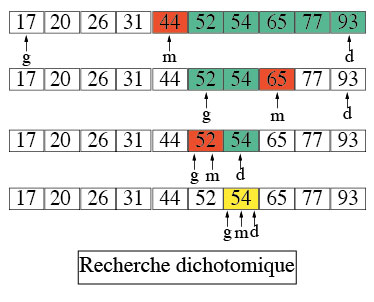
\includegraphics[width=0.4\textwidth]{dicho.jpg}
	\end{figure}
	\begin{lstlisting}[caption={Recherche dichotomique tableau trie}]
//Recherche dichotomique tableau trie
int rechercheDichotomique(Pile &pile, int val, int taille){
    int iDeb = 0; //indice debut du tableau de debut de recherche
    int iFin = pile.NbElts - 1; // indice du tableau de fin de recherche
    int iMil; // indice du tableau de milieu de recherche
    int index=-1;
    bool trouve = false;
    
    while( iDeb <= iFin && !trouve){
        iMil=(iDeb+iFin)/2;//calcul de l'indice milieu
        //cas ou la valeur est au milieu
        if (pile.Elts[iMil]==val){
            trouve=true;
            index=iMil;
        }
        //si ma valeur est avant le milieu, je cherche dans 1ere moitie
        else if (pile.Elts[iMil] > val){
            iFin = iMil - 1;
        }
        //si ma valeur est apres le milieu, je cherche dans 2eme moitie
        else if(pile.Elts[iMil] < val){
            iDeb = iMil +1;
        }
    }
    return index;
}
    \end{lstlisting}
\section{Utilisation d’une pile : Application}
\textbf{Ecrire} un algorithme qui vérifie qu’un texte contenant des caractères standards est syntaxiquement correct du point de vue des parenthèses.

Les parenthèses sont de trois types : \texttt{ (, \{, [ } et leurs parenthèses fermantes correspondantes sont respectivement \texttt{), \}, ]}.
$\rightarrow$ on peut commencer juste par les parenthèses
\begin{lstlisting}[caption={Rappel : Déclaration d'une chaîne de caractères},label=stringrappel]
char x[] = "une chaine de caractères avec des parenthèses ())())))))(((())";
cout << x[0] << endl;//la console affiche : u
int tailleChaine= strlen(chaine); // recupere la taille de la chaine
cout << tailleChaine << endl;//la console affiche : 78
\end{lstlisting}

La correction syntaxique implique qu’à chaque parenthèse ouvrante corresponde une parenthèse fermante du même type, plus loin dans le texte.


Le texte compris entre ces deux parenthèses devra également être correct du point de vue des parenthèses.

\begin{lstlisting}[caption={Aide pour Verification syntaxe},label=aide]
//permet de verifier que les caracteres forment des paires ouvrantes et fermantes
bool sontDesPaires(char ouvrant,char fermant){
    bool sontDesPaires = false;
    if(ouvrant=='(' && fermant == ')'){
        sontDesPaires = true;
    }else if(ouvrant=='{' && fermant == '}'){
        sontDesPaires = true;
    }else if(ouvrant=='[' && fermant == ']'){
        sontDesPaires = true;
    }
    return sontDesPaires;
}

bool verificationSyntaxe(char chaine[], Pile &pile){
    int tailleChaine= strlen(chaine); // recuperer la taille de la chaine passée en paramètre
    cout << "Verification syntaxe en cours ..."<<endl;
    cout<< "Longueur : "<<tailleChaine<<" "<<endl;
    cout<< "Chaine : "<< chaine <<endl;
    //parcours de la chaine de caractères
    for(int i =0;i<tailleChaine;i++)
    {
        //recupere le caratère courant
        char current = chaine[i];
        if(current == '(' || current == '{' || current == '['){ //verifie si c'est un caractère spécial ouvrant
            empiler(pile,current); //si oui, on ajoute ce caractere à la pile
        }
        else if(current == ')' || current == '}' || current == ']') //verifie si c'est un caractère spécial fermant
        {
            //verifie si la pile n'est pas vide
            //ou si le dernier caractère de la pile et le caractère courant forment une paire ouvrant/fermant
            if(estVide(pile)){
                //pile vide rien à verifier
                cout << "Erreur: Pas d'ouvrant pour: '"<< current << "' à l'index "<< i <<endl;
                return false;
            }else if(!sontDesPaires(queue(pile),current)){
                cout << "Erreur: Pas de fermant pour: '"<< queue(pile) << "' à l'index "<< i <<" avant '" << current<<"'."<<endl;
                return false;
            }else{
                depiler(pile);
            }
            /*
              if(!estVide(pile) && sontDesPaires(queue(pile),current)){
                depiler(pile); //si oui, on sait que la paire est bien formée on peut supprimer le dernier caractère de la pile pour passer à l'ouvrant précédent
             }else{
             sinon ça veut dire que la pile est vide ou que le dernier caractère et le courant ne forment pas de paire. Dans tous les cas, on ne peut plus faire le checking des ouvrants/fermants donc on retourne faux
               return false;
             }
             */
        }
    }
    //on retourne le boolean correspondant à savoir si la pile est vide: si vrai ça indiquera que les paires sont bien formées, sinon qu'il y a eu une erreur
    return estVide(pile);
}
\end{lstlisting}

\begin{lstlisting}[caption={Exemple de main pour verifier la syntaxe},label=main]
int main(){
    char a[] = "()";
    char b[] = "(()";
    char c[] = "())";
    char d[] = "(())";
    char e[] = "une chaine de caractères avec des parenthèses ())())))))(((())";
    char f[] = "([{)";
    char g[] = "([{])";
    char h[] = "([{[()]}])";
    bool chaineValide=false;
    Pile p;
    p = initPile();
    chaineValide=verificationSyntaxe(a, p); // bien formé
    afficherResultat(chaineValide);
    chaineValide=verificationSyntaxe(b, p); //mal formé
    afficherResultat(chaineValide);
    //...
    
    cin.get();//attendre que l'utilisateur appuie sur ENTREE
    return 0;
}
\end{lstlisting}

\end{document}